\documentclass[11pt,a4paper]{article}
\usepackage{amsmath}
\usepackage{amsfonts}
\usepackage{amssymb}
\usepackage{enumitem}
\usepackage{graphicx}

\usepackage{geometry}
\geometry{a4paper,left=2cm,right=2cm,top=1cm,bottom=1cm}

\begin{document}
	\begin{center}
		Data Science
		
		Ruichun Liu
		
		Problem Set 6
	\end{center}
\begin{enumerate}



    \item \textbf{Question 3}
		  \begin{description}
	            1. I download my Dataset from NYC Taxi & Limousine Commission,\\https://www1.nyc.gov/site/tlc/about/aggregated-reports.page.\\
	            2. I transform the date type so that I can draw a graph.\\
	            3. I use ggplot to draw three pictures for Trips.Per.Day,Unique.Drivers,and Unique.Vehicles by using geom\_line(), geom\_point(), and geom\_jitter() respectively.
          \end{description}
          
    \item \textbf{Question 5}
		  \begin{description}
		  The following pictures show the time trend of Trips.Per.Day,Unique.Drivers,and Unique.Vehicles for Black car, High Volume, Livery, Lux Limo, Green taxi and Yellow taxi. Now I am still struggling with showing date on the pictures by using "scales".
             \begin{figure}[h]
                 \centering
                 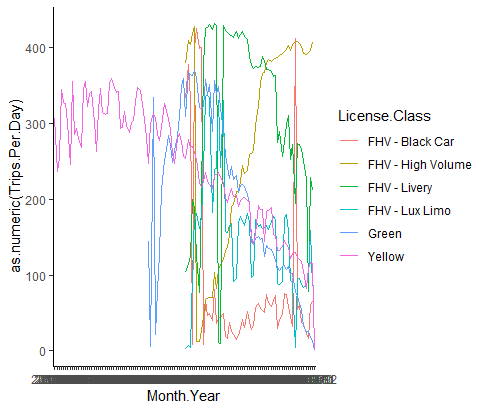
\includegraphics[width=14cm]{PS6a_LIU.png}
              \end{figure}
              
              \begin{figure}[p]
                 \centering
                 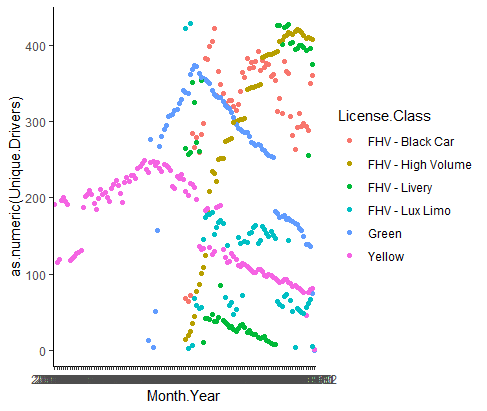
\includegraphics[width=14cm]{PS6b_LIU.png}
                 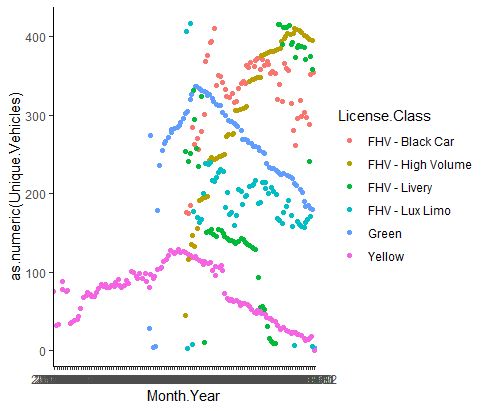
\includegraphics[width=14cm]{PS6c_LIU.png}
              \end{figure}
              
          \end{description}       

          
\end{enumerate}
\end{document}